\scanpage{18}
\mspage{32}

\margin{\figure{\begin{tikzpicture}\draw (.2,0)--(0,0)--(0,5)--(.2,5);\end{tikzpicture}}}
\uline{Corollaire} \inserted{4.}13. Soit $A\longrightarrow B$ un homomorphisme local d'anneaux locaux
noethériens, on suppose $k(B)/k(A)$ à multiplicité radicielle finie
(par exemple une extension séparable, ou de type fini),
\inserted{ou $\underline{r}(B)=\underline{r}(A)B$.} \deleted{Conditions} On
munit $A$ et $B$ de leurs topologies habituelles. Alors les conditions suivantes
sont équivalentes: (i) $B$ est formellement simple sur $A$ (ii) $B$ est
plat sur $A$, et $B_0=B\otimes_A k\deleted{\unsure{A}}$ est une algèbre universellement régulière sur
$k$ (cf 2.6.).

En effet, les conditions (i) et (ii) étant invariantes par changement
de $B$ en $\widehat{B}$, on est ramené au cas où $B$ est complet, où cela est contenu
dans \inserted{4.}11. \inserted{resp. \unsure{3.12.|4.12.}} compte tenu que pour $B_0$, formellement simple = universellement
régulier en vertu de \inserted{3.}6.

Du point de vue pratique, les résultats du présent numéro consistent
essentiellement en \inserted{4.}13., \deleted{l'existence}\deleted{et} l'\uline{unicité} \deleted{de $B$} (moyennant les conditions
de \inserted{4.}13.) du $B$ correspondant à un $B_0$ donné, sous réserve que $B$ soit
complet pour la topologie $\underline{r}(A)$-adique (cette \deleted{unici} unicité étant un
corollaire immédiat d'ailleurs, puisqu'on dispose pour $B$ des deux propriétés
complémentaires formellement simple + plat),
\inserted{et enfin l'\uline{existence} moyennant la séparabilité de $K/k$.}
A force de dévissage et
de généralité, cette substance n'apparait pas assez clairement, et la
terminologie ``algèbre de Cohen'' introduite concurremment à ``formellement
simple'' risque \deleted{peut-être} d'embrouiller \inserted{plutôt} les idées (d'autant plus que nous
n'utiliserons plus jamais que ``formellement simple'' ). Aussi le présent
numéro rendra peut-être plus service si on commence à énoncer simplement
\inserted{4.}13. en théorème, avec le corollaire bien senti précédent, et qu'on
les démontre simultanément en deux pages ou trois, \deleted{avec} en laissant de
côté tout le fatras anneaux admissibles, algèbres de Cohen etc. Commencer
par l'existence d'un $B$ satisfaisant à la fois (i) et (ii) si $K/k$ est
séparable, se ramener à ce cas pour \inserted{4.}13. par descente comme dans \inserted{4.}11.
prouver \inserted{4.}13. alors par comparaison du $B$-type avec le $B$ donné, ce qui
donne en même temps l'unicité, et un point c'est tout.

\margin{(garder cependant 4.1. \uuline{au \unsure{N°1}})
On peut signaler 4.6. en remarque, pour réserver l'avenir.}
\margin{\figure{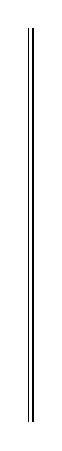
\begin{tikzpicture}\draw (0,0)--(0,5);\draw (.06,0)--(.06,5);\end{tikzpicture}}}

\mspage{17}
